\documentclass{vc}

\title{Visual Computing論文テンプレート}

\usepackage{tabularx}
\author{%
  {\large%
    \begin{tabularx}{.8\textwidth}{*3{>{\centering\arraybackslash}X}}
      画像 花子$^\dagger$ & 電子 太郎$^\ddagger$ & 学会 三郎$^\ddagger$
    \end{tabularx}
  }
  \\
  \begin{tabular}{cc}
    $\dagger$画像大学工学部 & $\ddagger$画像株式会社開発部
  \end{tabular}
  \\
  \begin{tabular}{c}
    E-mail: $\dagger${}hanako@gazo.ac.jp, $\ddagger${}\{taro, saburo\}@denshi.co.jp
  \end{tabular}
}

\begin{abstract}
  コンピュータ・グラフィックス(CG),及び,CGの周辺分野における革新的な技術の発表を募集します.
  創造的,独創的な学術的成果をはじめ,CG技術の新しい使い方や実用例などの応用的成果まで,未来のCG業界を刺激する幅広い投稿をお待ちしております.
\end{abstract}

\begin{teaserfigure}
  \centering
  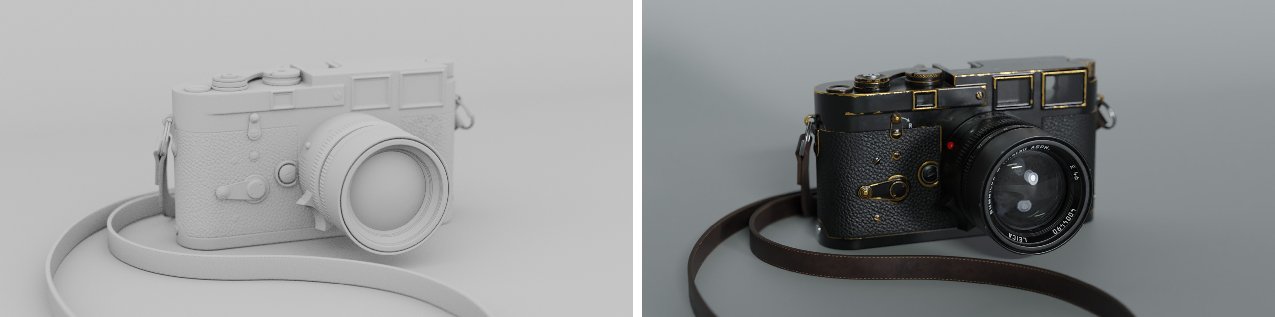
\includegraphics[width=\textwidth]{./figures/leica.pdf}
  \captionof{figure}{ティザー画像のキャプションをここに記述する.}
  \label{fig:teaser}
\end{teaserfigure}

\begin{document}

\maketitle

\section{VC 2020論文募集}

\subsection{はじめに}

コンピュータ・グラフィックス(CG),及び,CGの周辺分野における革新的な技術の発表を募集します.
創造的,独創的な学術的成果をはじめ,CG技術の新しい使い方や実用例などの応用的成果まで,未来のCG業界を刺激する幅広い投稿をお待ちしております.

募集するカテゴリは,論文(査読有り,口頭発表)とポスター(査読無し)の2つです.

論文に著者名,所属,謝辞などは書かないでください.WordからPDFを作成した場合,文書のプロパティに著者を特定できる情報が入ることがありますが,そのような情報は削除してください.

論文は締切前であれば何度でもアップロードできます.締切を過ぎた投稿は受け付けませんので,時間に余裕を持って投稿してください.

\subsection{論文(査読有り,口頭発表)}

学術的な研究成果について,研究の背景,理論,アルゴリズム,結果などを紹介する論文を募集します. また,CG技術の新しい使い方や,CG技術の産業応用に関する論文の投稿も歓迎します.投稿論文はプログラム委員会での議論を通じて,ロング発表,ショート発表,不採択のいずれかに判定されます.
また,ロング・ショートを問わず,採択論文は査読付きシンポジウム論文(フルペーパー)として扱います.

優秀なロング発表論文にはVC論文賞を,優秀なショート発表にはVCショート発表賞をそれぞれ授与します. 受賞論文にはそれぞれ賞状と副賞を贈呈するとともに,2020年夏頃に発行されるCGWORLD.jpに掲載予定の「Visual Computing 2020開催レポート」(仮題)の中で論文紹介されます.

\subsection{ポスター(査読無し)}

完成された研究のみならず,新しいアイデア,進行中の研究紹介など,さまざまな性格の発表を募集します.VCのポスターでは,「既存技術について,自分の頭で考え直したこと」もオリジナリティであるとして発表を歓迎します.優秀なポスターについてはVCポスター賞を授与します.

\section{テンプレートの使用例}
\label{sec:template}

本テンプレートを用いて原稿の本文を記述する際の例を下記に示す.
なお表の詳細なフォーマットや参照に用いるコマンド\footnote{ここでは\textsf{hyperref}パッケージが提供する\textsf{autoref}コマンド\cite{Wikibooks:LaTeX:Ref}を利用している.}などは厳密に従う必要はない.

インライン数式は$\mathbf{x} \in \mathbb{R}^{n}$のように記述する.
ディスプレイ数式は
\begin{align}
  \mathbf{A} \mathbf{x} = \mathbf{b}
  \label{eq:linear_system}
\end{align}
や, あるいは
\begin{align}
  \mathbf{x}^{*} = \mathop{\text{arg max}}_{\mathbf{x} \in \mathcal{X}} f(\mathbf{x})
\end{align}
などのように記述する.
数式は\autoref{eq:linear_system}などのように参照する.
図は\autoref{fig:teaser}や\autoref{fig:leica}などのように参照する.
表は\autoref{tab:accuracy}などのように参照する.
セクションは\autoref{sec:template}などのように参照する.
参考文献は\cite{GSC12,WL00}などのように参照する.
URLは\url{https://www.siggraph.org/}のように記載する.

\begin{figure}
  \centering
  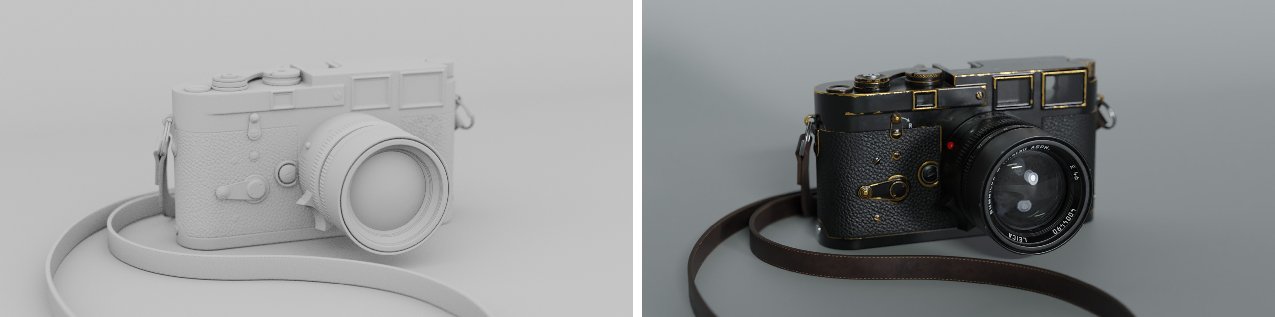
\includegraphics[width=\columnwidth]{./figures/leica.pdf}
  \caption{図のキャプションをここに記述する.}
  \label{fig:leica}
\end{figure}

\begin{table}
  \centering
  \caption{表のキャプションをここに記述する.}
  \label{tab:accuracy}
  \begin{tabular}{@{}rrrr@{}}
    \toprule
    & Our method & XXX et al. & YYY et al. \\
    \midrule
    Case 1 & \textbf{95.4\%} &         91.2\%  & 92.4\% \\
    Case 2 & \textbf{97.5\%} &         92.1\%  & 91.2\% \\
    Case 3 &         90.3\%  & \textbf{90.9\%} & 82.5\% \\
    \midrule
    Mean   & \textbf{94.4\%} &         91.4\%  & 88.7\% \\
    \bottomrule
  \end{tabular}
\end{table}

\bibliographystyle{IEEEtran}
\bibliography{template.bib}

\end{document}
